\chapter{Experiments}
\label{cha:Experiments}


\section{The Random Graph Model}
The random graph model we use for the experiment was inspired by the one introduced in \cite{toulis2011random}. It was designed for generating patient-donor pairs based on a fixed blood type distribution and tissue-type compatibility factor $1 - p_c = 0.8$. In our setting, we consider patient-donors groups with up to two proxy donors, so the already existing random graph model had to be modified in order to fit our requirements. We introduce a new variable; \textit{double donor ratio} ($ddr$), which represents the percentage of patient-donor groups with two proxy donors. The amount of information about what the value of $ddr$ is in the real-world KE programs is limited, \cite{holscher2018kidney} reports that only $7.3\%$ of candidates registered with more than one potential donor. The following are the algorithms we use for generating random patient-donor groups (\autoref{alg:generate_patient_donors}) and the compatibility edges between them (\autoref{alg:generate_compatibility_edges})

\begin{algorithm}
    \caption{Generate patient-donor groups with multiple donors}
    \label{alg:generate_patient_donors}

    \KwIn{$n$: number of patient-donor groups to generate, $ddr$: double donor ratio, $p_c$: tissue incompatibility factor}
    \KwOut{$D$: $n$ patient-donor groups}

    $D \gets \emptyset$\;
    $\#double\_donor\_groups \gets n \cdot ddr$\;
    \While{$|D| < n$}{
        $p \gets \text{pick random blood type}$\;

        \If{$|D| < \#double\_donor\_groups$}{
            $donor\_types \gets \text{pick 2 random blood types}$\;
        }
        \Else{
            $donor\_types \gets \text{pick 1 random blood types}$\;
        }
        \:

        \If{ $\forall d \in donor\_types$, $p$\textup{ is incompatible with }$d$ \textup{ or } $random() < p_c$ }{
            $D \gets D \cup \{(p, donors\_types)\}$\;
        }
    }
    \Return{D}
\end{algorithm}


\begin{algorithm}
    \caption{Generate compatibility edges}
    \label{alg:generate_compatibility_edges}

    \KwIn{$D$: patient-donor groups, $p_c$: tissue incompatibility factor}
    \KwOut{$E_c$: compatibility edges}

    $E_c \gets \emptyset$\;
    \ForEach{$(p_i, donors_i) \in D$}{
        \ForEach{$(p_j, donors_j) \in D$ where $i \neq j$}{
            \ForEach{$d \in donors_i$}{
                \If{$d$ \textup{ is blood type compatible with } $p_j$ \textup{ and } $random() \ge p_c$}{
                    $E_c \gets E_c \cup \{(p_j \rightarrow d)\}$\;
                }
            }
        }
    }

    \Return{$E_c$}
\end{algorithm}

The graph we generate can be adapted to the model with only one donor per group by either randomly removing one of the proxy donors from each group containing two proxy donors, or by setting the parameter $ddr$ to $0$ (which is equivalent to the model described in \cite{toulis2011random}). Importantly, these two methods produce models of KE programs with different blood type distributions. Notably, as $ddr$ increases, the percentage of patients with an unfavorable blood type O also increases, as shown in \autoref{fig:patient_blood_type_as_ddr_increases}.

\begin{figure}[H]
    \centering
    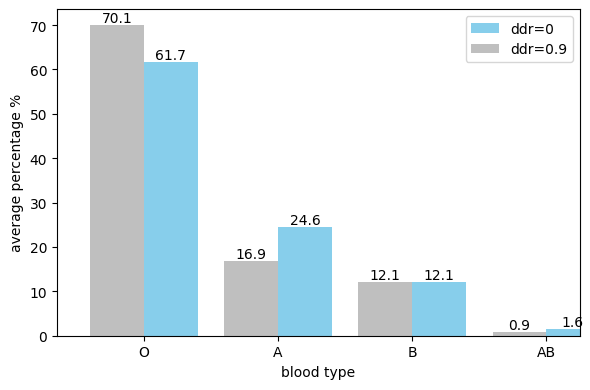
\includegraphics[width=1.\linewidth]{data/patient_blood_type_as_ddr_increases.png}
    \caption[Distribution of patients' blood types as double donor ratio changes]{The diagram illustrating the change in the distribution of patients' blood types in KE programs as we change the ratio of groups having two proxy donors.}
    \label{fig:patient_blood_type_as_ddr_increases}
\end{figure}


\section{Experiment Overview}

In this section, we present the experimental evaluation of our proposed model. We aim to investigate the practical impact of allowing multiple donors per patient under different kidney exchange settings.

Our focus is on the \textit{2-Cycle 1-Chain Multi-Donor Kidney Exchange Model}. For comparison, we include \textit{2-Cycle No-Chain Multi-Donor Model} (\textit{Alternative-Donors Model}), where each patient may have up to two donors, but at most one donor can be used, and only 2-cycles are allowed.

We then formulate the resulting problem as an instance of integer programming introduced in \autoref{sec:Integer Linear Program Formulation} and solve it using IBM ILOG CPLEX Optimizer~\cite{cplex}.

CPLEX is capable of computing optimal solutions efficiently in most cases; however, it does not guarantee short runtimes for all instances. Therefore, we set a timeout threshold: if a single task runs for more than 12 minutes, it is terminated and excluded from the results.


For the experimental analysis, we investigate two key questions.
\begin{experiment}
    \label{exp:percentage_vs_number_of_patients}
    \textup{We examine how the percentage of patients matched changes as the total number of patients increases across the two models. We expect the match rates for both of them to increase slightly as the number of patients grows, due to more potential matches being available. However, we do not expect a significant increase, since the compatibility graph is already fairly dense. We expect that as the number of patients increases, the variance will decrease.}
\end{experiment}

\begin{experiment}
    \label{exp:percentage_vs_ddr}
    \textup{
    We analyze how the match rate varies with the proportion of patients having a second donor. Specifically, we hypothesize the following trends:
    \begin{itemize}
    \item For the \textit{2-Cycle No-Chain Multi-Donor Model}, the effect is ambiguous: while the increased donor pool may improve match opportunities, the changing distribution may counteract this benefit.
    \item For the \textit{2-Cycle 1-Chain Multi-Donor Model}, we expect a clear increase in the match rate, as the additional donors provide more opportunities to initiate chains.
    \end{itemize}
    }

\end{experiment}



\section{Results}


The following two figures (\autoref{fig:test2} and \autoref{fig:test}) present the experimental results. The semi-transparent region around the curve indicates the variance across runs. For each test case, we run the experiment 100 times and average the results.
In the first experiment, the number of patients is fixed at 1000. In the second experiment, the double donor rate is fixed to $10\%$.

As expected, all observed trends are consistent with our hypotheses. In \autoref{exp:percentage_vs_number_of_patients}, the \textit{2-Cycle 1-Chain Multi-Donor Model} achieves an improvement over the \textit{2-Cycle No-Chain Multi-Donor Model}, increasing the match rate by $5\%$ for all numbers of patients. In \autoref{exp:percentage_vs_ddr}, interestingly, when $ddr$ reaches $10\%$, the percentage of saved patients in the \textit{2-Cycle 1-Chain Multi-Donor Model} converges to $60\%$, achieving a $5\%$ increase over the \textit{2-Cycle No-Chain Multi-Donor Model}.

\begin{figure}[H]
    \centering
    \includesvg[width=\linewidth]{data/test2}
    \caption[Average percentage of satisfied patients vs number of patients (with double donor ratio = 0.1)]{Results of \autoref{exp:percentage_vs_number_of_patients}. Average percentage of satisfied patients vs number of patients (with double donor ratio = 0.1)}
    \label{fig:test2}
\end{figure}

\begin{figure}[H]
    \centering
    \includesvg[width=\linewidth]{data/test}
    \caption[Average \% of satisfied patients (among 1000) vs double donor ratio]{Results of \autoref{exp:percentage_vs_ddr}. Average \% of satisfied patients  (among 1000) vs double donor ratio}
    \label{fig:test}
\end{figure}


Regarding computational efficiency, we observe that for most instances (up to one thousand patients), the optimal solution can be computed within one minute on a standard laptop. More specifically, out of 1,100 instances, only four exceeded the timeout threshold. This indicates that computational resources are unlikely to pose a practical bottleneck for applying our model in real-world scenarios.


%%% Local Variables:
%%% mode: latex
%%% TeX-master: "../ClassicThesis"
%%% ispell-dictionary: "british" ***
%%% fill-column: 76 ***
%%% End:
